%%%
%%% Improved Datahandling
%%%
\part{Improved Datahandling}
\begin{frame}
\thispagestyle{empty}
\textbf{\huge{Improved\\ Datahandling}}
\end{frame}

\begin{frame}{Improved\\ Datahandling Contents}
 \tableofcontents
\end{frame}

\section{by}
\begin{frame}[fragile]{by I} \index{by} \index{by!bysort}
Select subsets
\begin{lstlisting}
  summarize weight if sex == 1
  summarize weight if sex == 2
\end{lstlisting}

Do it in a single line
\begin{lstlisting}
  by edu, sort: summarize hhinc
\end{lstlisting}

  \begin{tikzpicture}[transform shape, rotate=10, overlay]
\node at (7.5,-0.5) [mybox] (box) {%
    \begin{minipage}[t!]{0.35\textwidth}
    \tiny\textcolor{black}{\texttt{by is not allowed with every command, in doubt contact the help. To use by cases have to be sorted. Alternativ: bysort}}
    \end{minipage}
    };
\end{tikzpicture}
\end{frame}

\begin{frame}[fragile]{by II}
Es können auch mehrere Variablen genommen werden \index{by}
\begin{lstlisting}
  by sex county, sort: summarize weight
\end{lstlisting}
\end{frame}

\section{in}
\begin{frame}[fragile]{in}
Select only a few cases \index{list}
\begin{lstlisting}
  ** select the first
  list sex in 1
  ** select the first ten
  list sex in 1/10
\end{lstlisting}

  \begin{tikzpicture}[transform shape, rotate=10, overlay]
\node at (7.5,-0.5) [mybox] (box) {%
    \begin{minipage}[t!]{0.35\textwidth}
    \tiny\textcolor{black}{\texttt{Usually single cases are not interesting, but this can be helpful to spot strange cases.}}
    \end{minipage}
    };
\end{tikzpicture}
\end{frame}


\section{Loops}
\begin{frame}[fragile]{Loops I} \index{Loops} \index{Loops!foreach}
Loops in Stata. Example from \textcite[69f.]{Kohler2012}
\begin{lstlisting}
** Generate variables r1 - r10
** Newlist
foreach var of newlist r1-r10 {
  gen `var' = runiform()
}

** Numeric list
foreach num of numlist 1/10 {
  replace r`num' = runiform()
}
\end{lstlisting}
\end{frame}

\begin{frame}[fragile]{Loops II} \index{Loops} \index{Loops!foreach} \index{Loops!forvalues}
\begin{lstlisting}
** multiple commands in a loop
foreach var of varlist ybirth income {
  summarize `var', meanonly
  generate `var'_c = `var' - r(mean)
  label variable `var'_c "`var' (centered)"
}
\end{lstlisting}

\begin{lstlisting}
** Forvalues
forvalues num = 1/10 {
  replace r`num' = runiform()
}
\end{lstlisting}
\end{frame}

\section{log-files}
\begin{frame}[fragile]{log-files} \index{log} \index{log!log-files}
  \begin{itemize}
    \item Results can be stored in log-files.
    \item These contain all commands and their results.
    \item Logging begins after
    \begin{lstlisting}
  log using <dateiname.log>
    \end{lstlisting}
    \item log-files can be opened with every texteditor.
  \end{itemize}
\end{frame}

\begin{frame}[fragile]{log-files II}
  \begin{itemize} \index{log} \index{log!using} \index{log!close}
   \item Define a name and path where the log-file is saved. Usually the log-file name should reflect the do-files name.
   \begin{lstlisting}
  log using read-soep.log, replace
   \end{lstlisting}
   \item At the end of the do-file
   \begin{lstlisting}
  ** commands will not be logged after this
  log close
   \end{lstlisting}
   \item Thrown errors stop the do-files execution, therefore a manual closing of the log-file might be required because Stata cannot handle two open log-files
   \begin{lstlisting}
  log close
   \end{lstlisting}
  \end{itemize}
  
    \begin{tikzpicture}[transform shape, rotate=10, overlay]
\node at (7.5,-0.5) [mybox] (box) {%
    \begin{minipage}[t!]{0.35\textwidth}
    \tiny\textcolor{black}{\texttt{capture log close atop log using ensures that all open log-files will be closed.}}
    \end{minipage}
    };
\end{tikzpicture}
\end{frame}

\section{Macros}
\begin{frame}[fragile]{Macros} \index{Macros} \index{Macros!global}
With longer pathes and bigger projects it is helpful to use so called Macros. Macros may be global (it is known everywhere inside your code) or local (it is known only in a specific loop). We use macros for paths
\begin{lstlisting}
  ** global Macroname Pathname
  global DATA "D:/Data/data/original/"
  global OUT "D:/Data/data/bearbeitet/"
\end{lstlisting}
Now the macros can be called like this
\begin{lstlisting}
 cd "${DATA}"
\end{lstlisting}

\end{frame}

\begin{frame}[fragile]{Macros II}
It is especially helpfull handling long or different directorys for input, output, images or log files. Some additional examples \index{Macros}
\begin{lstlisting}
  use "${DATA}testdata.dta", clear
  save "${OUT}testdata_recoded.dta", replace
\end{lstlisting}
The syntax readability benefits a lot from this

  \begin{tikzpicture}[transform shape, rotate=10, overlay]
\node at (7.5,-2.1) [mybox] (box) {%
    \begin{minipage}[t!]{0.35\textwidth}
    \tiny\textcolor{black}{\texttt{Your saving time. Long paths are written once, which minimizes typos. A correct macros is correct for the full document. Still macros don't help you with thinking.}}
    \end{minipage}
    };
\end{tikzpicture}

\end{frame}

\section{Using}
\begin{frame}[fragile]{using} \index{Import!use using} \index{Sort!sort}
Stata can handle only a limited range of variables, so a little housekeeping is advised.\footnote{Different Stata versions have different limits: IC (the version your working with) can handle $2,047$, SE can handle $32,767$ variables. Handling more variables is rather expensive. Prices for 2013: \$189 and \$395 for students. Non academic single user licenses \$$1545$ and \$$2090$.} Handling the SOEP this limit is not as far away as you might believe.
\begin{lstlisting}
  ** Import a minimal ppfad
  ** kepp only hhnr persnr sex gebjahr
  use hhnr persnr sex gebjahr using "${DATA}ppfad.dta"
  ** Sort cases by persnr and gebjahr
  sort persnr gebjahr
\end{lstlisting}
\end{frame}

\section{Merge}
\begin{frame}{merge} \index{Merge!merge}
\begin{minipage}{11cm}
In the Sozio-oekonomischen Panel (SOEP) (s. \cite{Wagner07}) each years data is split into different smaller data files. This has historical and maybe even practical reasons.\\
Starting from a file different of these data files share, we can combine the smaller files to generate a complete data set. This combination is called \textit{merging}.
\end{minipage}
\end{frame}

\begin{frame}[fragile]{merge II} \index{Merge!merge}
\begin{minipage}{11cm}
As example: We merge \textbf{ppfad} with \textbf{bep} and \textbf{bepgen}. \textbf{ppfad} is the data file ever person file shares. To make sure that we combine only persons data correct, we seek for matches of household-id (hhnr) and person-id (persnr).\\

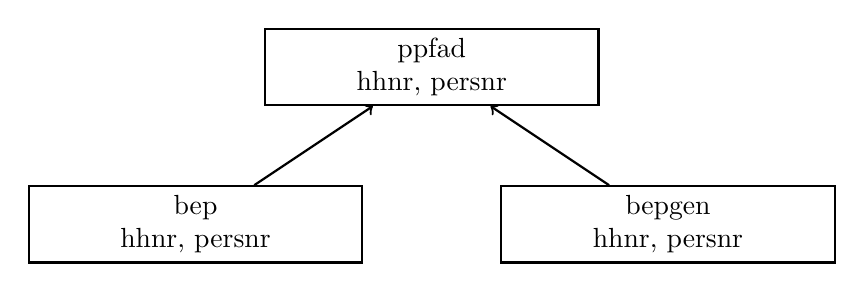
\begin{tikzpicture}[thick]
\node at ( 3,2) [rectangle,draw=black,text width=4cm,align=center] (ppfad) {ppfad \\
									    hhnr, persnr};

\node at ( 0,0) [rectangle,draw=black,text width=4cm,align=center] (bekind) {bep \\
									    hhnr, persnr};
\node at ( 6,0) [rectangle,draw=black,text width=4cm,align=center] (bepgen) {bepgen \\
									    hhnr, persnr};
									    
\draw[->] (bekind) -- (ppfad);
\draw[->] (bepgen) -- (ppfad);
\end{tikzpicture}
\end{minipage}
\end{frame}


\begin{frame}[fragile]{merge III}
Running \texttt{merge} \index{Merge!merge}

\begin{lstlisting}
  ** merge ppfad with 2014 bep
  merge 1:1 persnr using "${DATA}bep.dta"
\end{lstlisting}

\begin{table}
\begin{center}
\begin{scriptsize}
\begin{tabular}{lll}
 Result & \# of obs. & \\ 
 \midrule
 not matched & 25,834 & \\
 ~~from master & 25,834  &(\_merge==1) \\
 ~~from using  & 0 &(\_merge==2) \\
 & & \\
 matched & 10,471 & (\_merge==3) \\
 \midrule
\end{tabular}
\end{scriptsize}
\end{center}
\end{table}
This means 
\begin{itemize}
 \item $25,834$ cases of \texttt{ppfad} were not found in \texttt{bep}.
 \item $0$ cases of \texttt{bep} were not found in \texttt{ppfad}
 \item $10,471$ cases of \texttt{bep} were found in \texttt{ppfad}
\end{itemize}
\end{frame}

\begin{frame}[fragile]{merge IV}\index{Merge!\_merge}\index{Merge!merge}
\begin{minipage}{11cm}
A new variable \texttt{\_merge} is created containing the \texttt{\_merge==} values. For now we remove all cases where we could not find a match from \texttt{using} which is \texttt{\_merge==2}. These are potentially problematic as we have no information about these persons sex or year of birth. Lucky at our current stage these are zero cases. Afterwards we remove \texttt{\_merge}.
\begin{lstlisting}
  ** Drop if using does not match master
  drop if _merge==2
  ** drop _merge
  drop _merge
\end{lstlisting}
\end{minipage}


  \begin{tikzpicture}[transform shape, rotate=10, overlay]
\node at (7.5,-1.5) [mybox] (box) {%
    \begin{minipage}[t!]{0.35\textwidth}
    \tiny\textcolor{black}{\texttt{The coice which merge is dropped is depending on the analysis.}}
    \end{minipage}
    };
\end{tikzpicture}

\end{frame}

\begin{frame}[fragile]{merge V} \index{Merge!merge} \index{Merge!merge, keepusing}
Example: merge with the generated variable highest educational achievement \texttt{bepsbil} from data-file \textbf{bepgen}.

\begin{lstlisting}
  merge 1:1 hhnr persnr using "${DATA}bepgen.dta", keepusing(bepsbil)
  drop if _merge==2
  drop _merge
\end{lstlisting}

  \begin{tikzpicture}[transform shape, rotate=10, overlay]
\node at (7.5,-1.5) [mybox] (box) {%
    \begin{minipage}[t!]{0.35\textwidth}
    \tiny\textcolor{black}{\texttt{In \textbf{bepgen} contains $65$ variables, but all we need is the educational achievement.}}
    \end{minipage}
    };
\end{tikzpicture}
\end{frame}

\section{Operators}
\begin{frame}[fragile]{Operators} \index{Operators}
Stata list the following operators, which can be used with variables. Using \texttt{var1\^{}2} every value of \texttt{var1} will be squared.
\begin{lstlisting}
 == // equals
 != // not equal ~=
 & // and
 | // or
 ! // not
 < // smaller
 > // greater
 <= // smaller equal
 >= // greater equal
 + // plus
 - // minus
 / // divide
 * // mutiply
 ^ // power
\end{lstlisting}
\end{frame}

\begin{frame}[fragile]{Functions} \index{Functions}
Additionaly Stata contains a range of built in functions (\texttt{help functions}).
A selection:
\begin{lstlisting}
  abs() // absolute value/modulus |-2| == 2
  max() // greates value
  min() // smalles value
  exp() // e-function
  ln() // logarithm
  round() // round
  sin() // Sinus
  sqrt() // square root
  runiform() // random number
\end{lstlisting}
\end{frame}